% Welcome! This is the unofficial University of Udine beamer template.

% See README.md for more informations about this template.

% This style has been developed following the "Manuale di Stile"
% (Style Manual) of the University of Udine. You can find the
% manual here: https://www.uniud.it/it/ateneo-uniud/ateneo-uniud/identita-visiva/manuali-immagine-stile/manuale-stile

% Note: for some reason, the RGB values specified in the manual
% do NOT render correctly in Beamer, so they have been redefined
% for this document using the high level chromo-optic deep neural 
% quantistic technology offered by Microsoft Paint's color picker.

% We defined four theme colors: UniBrown, UniBlue, UniGold
% and UniOrange. For example, to write some uniud-brownish
% text, just use: \textcolor{UniBrown}{Hello!}

% Note that [usenames,dvipsnames] is MANDATORY due to compatibility
% issues between tikz and xcolor packages.

\documentclass[usenames,dvipsnames,table]{beamer}
\usepackage[utf8]{inputenc}
\usepackage{verbatim}
\usetheme{uniud}


%%% Bibliography
\usepackage[
  backend=biber,
  style=numeric,
  citestyle=numeric,
  giveninits=true,
  eprint=false,
  url=false,
  doi=false,
  isbn=false
]{biblatex}
\addbibresource{bibliography.bib}

% Author names in publication list are consistent 
% i.e. name1 surname1, name2 surname2
% See https://tex.stackexchange.com/questions/106914/biblatex-does-not-reverse-the-first-and-last-names-of-the-second-author
\DeclareNameAlias{author}{given-family}

%%% Suppress biblatex annoying warning
\usepackage{silence}
\WarningFilter{biblatex}{Patching footnotes failed}

%%% Some useful commands
% pdf-friendly newline in links
\newcommand{\pdfnewline}{\texorpdfstring{\newline}{ }} 
% Fill the vertical space in a slide (to put text at the bottom)
\newcommand{\framefill}{\vskip0pt plus 1filll}


\title[University of Udine]{\LARGE Comparison of Tools for the Verification of Cryptographic Protocols}
\date[September 2021]{\small September 20, 2021}
\author[Alessandro Zanatta]{\small
  Alessandro Zanatta,
  \pdfnewline
  Bachelor in Internet of Things, Big Data and Web
}
\institute{\small Course in Computer Network Security}

%% -------------------------------------------------------------------------------- %%
%% Additional packages                                                              %% 
%% -------------------------------------------------------------------------------- %%
\usepackage{listings}
\usepackage{cleveref}
\usepackage{afterpage}
\usepackage{msc}
\usepackage[euler]{textgreek}
\usepackage[justification=centering]{caption}
\usepackage{courier}
\usepackage{tikz}
\usepackage{array}
\usepackage{pifont}
\usepackage{multirow}
\usepackage{ctable}
\usepackage{booktabs}
\usepackage{changepage}
\usepackage{caption}
\usepackage{soul}
\usepackage{multicol}

\graphicspath{{logos/},{images/}} % Images folder(s)

\captionsetup{skip=0pt}
\setbeamercolor{alerted text}{fg=white}
\sethlcolor{UniOrange}
\renewcommand<>{\hl}[1]{\only#2{\beameroriginal{\hl}}{#1}}
\makeatletter
\let\HL\hl
\renewcommand\hl{%
  \let\set@color\beamerorig@set@color
  \let\reset@color\beamerorig@reset@color
  \HL}
\makeatother
\SoulColor

\setbeamercovered{transparent}

%% -------------------------------------------------------------------------------- %%
%% Commands                                                                         %%
%% -------------------------------------------------------------------------------- %%

% Highlight text
\newcommand<>{\myhl}[1]{\alert#2{\hl#2{#1}}}

% Checkmark and cross
\newcommand{\cmark}{\ding{51}}
\newcommand{\xmark}{\ding{55}}

% Basic setting for listings
\lstset{basicstyle=\scriptsize\ttfamily,breaklines=true,captionpos=b}

% msc options command
\newcommand\setmscoptions{%
  \setlength{\instdist}{1.5cm}%
  % \setlength{\levelheight}{1.5 \levelheight}%
  % \setlength{\instwidth}{3cm}
  \setmsckeyword{}
  \drawframe{no}
  \centering
}

\newcommand*{\Z}{\ensuremath{\mathbb{Z}}}
\newcommand*{\Q}{\ensuremath{\mathbb{Q}}}

%% Taken from https://hal.inria.fr/file/index/docid/955869/filename/sapic.tex
\newcommand{\msrewrite}[1]{\mathrel{-\hspace{-2pt}[#1]\hspace{-4pt}\to}}
\newcommand{\emptyrule}{\ensuremath{[]}\xspace}
\newcommand{\msr}[3]{\ensuremath{\left[#1\right] \msrewrite{#2} \left[#3\right]}}
%% -------------- %%

\newcommand{\msrfact}[2]{\ensuremath{\mbox{#1}\left(#2\right)}}

% Multiset rewriting rules
\newcommand{\msrnolabel}[2]{\ensuremath{#1 \rightarrow #2}}
\newcommand{\msrsetminus}{\ensuremath{\setminus^\#}}
\newcommand{\msrcap}{\ensuremath{\cap^\#}}
\newcommand{\msrcup}{\ensuremath{\cup^\#}}
\newcommand{\msrin}{\ensuremath{\in^\#}}
\newcommand{\msrsubseteq}{\ensuremath{\subseteq^\#}}

% Applied pi-calculus
\newcommand{\pic}{\textpi-calculus }
\newcommand{\picnospace}{\textpi-calculus}

% Cryptographic primitives
\newcommand{\func}[2]{\ensuremath{\mbox{#1}\left(#2\right)}}
\newcommand{\enc}[2]{\ensuremath{\left\{#1\right\}_{#2}}}
\newcommand{\sha}[2]{\ensuremath{\func{sha#1}{#2}}}
\newcommand{\kdf}[1]{\ensuremath{\func{kdf}{#1}}}
\newcommand{\fpk}[1]{\ensuremath{\func{fpk}{#1}}}
\newcommand{\hash}[1]{\ensuremath{\func{hash}{#1}}}
\newcommand{\modexp}[3]{\ensuremath{#1^#2 \mod{#3}}}
\newcommand{\key}[1]{\ensuremath{k_{#1}}}
\newcommand{\pkey}[1]{\ensuremath{pk_{#1}}}
\newcommand{\skey}[1]{\ensuremath{sk_{#1}}}
\newcommand{\newkey}[1]{\ensuremath{k'_{#1}}}
\newcommand{\group}[1]{\ensuremath{\Z_{#1}}}

% Circles
\newcommand*\emptycirc[1][1ex]{\tikz\draw[] (0,0) circle (#1);} 
\newcommand*\halfcirc[1][1ex]{%
  \begin{tikzpicture}
  \draw[fill] (0,0)-- (90:#1) arc (90:270:#1) -- cycle ;
  \draw (0,0) circle (#1);
  \end{tikzpicture}}
\newcommand*\fullcirc[1][1ex]{\tikz\fill (0,0) circle (#1);} 

%% -------------------------------------------------------------------------------- %%
%% Languages listings                                                               %%
%% -------------------------------------------------------------------------------- %%
\lstdefinelanguage{tamarin}
{
  keywordstyle=\color{MidnightBlue}\bfseries,
  keywordstyle=[2]\itshape,
  keywordstyle=[3]\color{Green}\bfseries,
  keywordstyle=[4]\color{RedViolet}\bfseries,
  keywords={Out, In, K, KU, Fr},
  keywords=[2]{},
  keywords=[3]{},
  keywords=[4]{rule},
  sensitive=true,
  morecomment=[l]{//},
  morecomment=[n][\color{OliveGreen}\itshape]{/*}{*/},
  morestring=[b]",
}

\lstdefinelanguage{verifpal}
{
  keywordstyle=\color{MidnightBlue}\bfseries,
  keywordstyle=[2]\itshape,
  keywordstyle=[3]\color{Green}\bfseries,
  keywordstyle=[4]\color{Orange}\bfseries,
  alsoletter={->, ?},
  keywords={principal, attacker, queries, ->, ?},
  keywords=[2]{Client, Server, Alice, Bob},
  keywords=[3]{leaks, phase},
  keywords=[4]{active, passive},
  sensitive=true,
  morecomment=[l]{//},
  morestring=[b]",
}

\lstdefinelanguage{proverif}
{
  keywordstyle=\color{MidnightBlue}\bfseries,
  keywordstyle=[2]\itshape,
  keywordstyle=[3]\color{Green}\bfseries,
  keywords={table, query, insert, leaks, phase, get, out, event, in, ., ;, attacker, |, new, if, else, then, !, let},
  alsoletter={., ;, |, !},
  keywords=[2]{Client, Server},
  keywords=[3]{},
  sensitive=true,
  morecomment=[l]{//},
  morecomment=[n][\color{OliveGreen}\itshape]{(*}{*)},
  morestring=[b]",
}

% Bibliography size
\renewcommand*{\bibfont}{\scriptsize}

%% -------------------------------------------------------------------------------- %%
%% Start of beamer document                                                         %%
%% -------------------------------------------------------------------------------- %%

\begin{document}

\begin{frame}
\titlepage
\end{frame}

\begin{frame}{Outline}
\tableofcontents
\end{frame}

\section{Why?}
\begin{frame}[t]{Why?}
  Cryptographic protocols are:
  \begin{itemize}
    \item{ubiquitous;}\pause
    \item{fundamental for security;}\pause
    \item{error-prone (e.g. Needham-Schroeder Public Key \cite{NSPK} and Lowe fix \cite{NSLPK}).}
  \end{itemize}

  \vskip 1cm

  \onslide<3->{Solution?}
  
  \onslide<4>{\begin{center}
    \LARGE\textbf{\textcolor{UniGold}{Formal verification of protocols!}}\par
  \end{center}}
  
\end{frame}

\section{How?}
\begin{frame}[t]{How?}
  Two possible models:
  \begin{itemize}
    \pause
    \item{\myhl<3->{Symbolic model};}
    \item{Computational model.}
  \end{itemize}

  \vskip 0.5cm

  \pause\pause
  Main elements:
  \begin{itemize}
    \pause
    \item{Attacker $\to$ Dolev-Yao \cite{DolevYao};}\pause
    \item{Cryptographic primitives $\to$ black-box;}\pause
    \item{Messages $\to$ terms.}\pause
    \item{\myhl{Perfect cryptography} assumption;}
  \end{itemize}

  \vskip 0.5cm
\end{frame}

\begin{frame}[t]{Perfect cryptography assumption example}

  Suppose we have:
  \begin{itemize}
    \pause
    \item{Two primitives: $\mbox{enc}$, $\mbox{dec}$;}\pause
    \item{Two terms: $m$, $k$;}\pause
    \item{The following equality:
      \begin{equation}
        \mbox{dec}\left(\mbox{enc}\left(m, k\right), k\right) = m
      \end{equation}
    }
  \end{itemize}

  \vskip 0.5cm

  \onslide<5>{
  Under the \textcolor{UniGold}{perfect cryptography} assumption: 
  \begin{center}
    can decrypt $\mbox{enc}\left(m, k\right) \Longleftrightarrow k$ is known
  \end{center}}
\end{frame}

\begin{frame}[t]{Available tools}
  Many tools:
  \begin{itemize}
    \item{\myhl<2->{Tamarin prover}}
    \item{\myhl<2->{Proverif}}
    \item{\myhl<2->{Verifpal}}
    \item{Scyther}
    \item{Scyther-proof}
    \item{AVISPA project}
    \item{Maude NPA}
    \item{... and others}
  \end{itemize}
\end{frame}

\section{Tamarin prover, Proverif and Verifpal}
\framecard{Tamarin prover,\\Proverif and Verifpal}  

\subsection{Tamarin prover}
\begin{frame}{Tamarin prover}
  Based on \cite{TamarinFoundations,TamarinManual}:
  \begin{itemize}
    \item{Protocol and adversary capabilities $\to$ \myhl<2->{Labelled multiset rewriting rules};}
    \item{Security properties $\to$ Guarded fragment of first order logic (with timepoints);}
    \item{Cryptographic primitives $\to$ Functions and equational theories;}
    \item{Verification $\to$ Constraint solving algorithm (backward-search and heuristics).}
  \end{itemize}
  
\end{frame}

\begin{frame}[fragile]{Labelled multiset rewriting rules}
  \lstset{language=tamarin}
  \begin{itemize}
    \item{Terms $\to$ can be thought of as messages;}
    \item{Facts $\to$ model information;}
    \item{Special facts $\to$ \lstinline{In(x)}, \lstinline{Out(x)}, \lstinline{Fr(x)} and \lstinline{K(x)};}
    \item{State $\to$ Multiset of facts;}
    \item{Transition rules $\to$ allows transitions between states.
    \begin{lstlisting}
rule ExampleRule:
    [ Fr(x) ]
  --[ ValueIsFresh(x)]->
    [ Out(x) ]
    \end{lstlisting}}
    \item{Trace $\to$ a sequence of (ground) facts denoting the sequence of actions happened.}
  \end{itemize}
\end{frame}

\begin{frame}{State transitions}
  \begin{block}{State transitions}
    Consider a ground multiset rewriting rule $\msr{l}{a}{r}$.

    If we call the state of the system $S$, the trace $T$ and assuming $l \msrsubseteq S$, the new state $S'$ is defined as:
    \begin{equation}
      S' = S \msrsetminus l \msrcup r
    \end{equation}
    Additionally, we append $a$ to the end of the current trace.
  \end{block}
\end{frame}

\subsection{Proverif}
\begin{frame}{Proverif}
  Based on \cite{ProverifFoundations}:
  \begin{itemize}
    \item{Protocol and adversary capabilities $\to$ \myhl<2->{\hbox{Applied \picnospace}};}
    \item{Security properties $\to$ Queries on events (resembles propositional logic);}
    \item{Cryptographic primitives $\to$ Constructors, destructors and equations;}
    \item{Verification $\to$ Resolution algorithm applied on the protocol translation to Horn clauses.}
  \end{itemize}
\end{frame}

\begin{frame}[fragile]{Proverif's applied \picnospace}
  \lstset{language=proverif}
  Grammar of processes ($P$, $Q$):
  \begin{lstlisting}
0                    (* null process *)
out(N, M); P         (* output to channel N the message M *)
in(N, M: T); P       (* input from channel N of message M *)
P | Q                (* parallel composition *)
!P                   (* infinite replication *)
new a: T; P          (* fresh value of sort T *)
if M then P else Q   (* conditional *)
  \end{lstlisting}
\vskip 0.5cm
  Additionally:
  \begin{lstlisting}
event EventName(x);        (* add event to trace *)
query event(EventName(x)). (* define a query on events *)
phase t;                   (* execute a process in phase t *)
let macroName = P.         (* create a process macro *)
let x = M in P else Q.     (* assignment and pattern matching *)
  \end{lstlisting}
\end{frame}

\subsection{Verifpal}
\begin{frame}{Verifpal}
  \lstset{language=verifpal,basicstyle=\footnotesize\ttfamily}
  Based on \cite{VerifpalManual,VerifpalFoundations}:
  \begin{itemize}
    \item{Protocol and adversary capabilities $\to$ \lstinline{principal} blocks and messages exchanges;}
    \item{Security properties $\to$ \lstinline{queries} block;}
    \item{Cryptographic primitives $\to$ pre-defined (no user-defined ones);}
    \item{Verification $\to$ Resolution algorithm in slide \ref{frame:verifpal-res-alg}.}
  \end{itemize}
\end{frame}

\begin{frame}[t,fragile]{Verifpal}
  Verifpal minimal working example:
  \lstset{language=verifpal,basicstyle=\scriptsize\ttfamily}
  \begin{lstlisting}
attacker [active]

principal Alice []
principal Bob []

queries []
  \end{lstlisting}

  \pause
  \lstset{language=verifpal,basicstyle=\footnotesize\ttfamily}
  Constructs:
  \begin{itemize}
    \item{\lstinline{attacker} $\to$ \lstinline{active} or \lstinline{passive};}\pause
    \item{Inside a \lstinline{principal} block:
      \begin{itemize}
        \item{\lstinline{generates}}
        \item{\lstinline{knows}}
        \item{\lstinline{leaks}}
        \item{assignments}
        \item{cryptographic primitives}
      \end{itemize}
    }\pause
    \item{\lstinline{queries} $\to$ confidentiality, authentication, freshness, unlinkability and equivalence.}
  \end{itemize}
\end{frame}

\begin{frame}[label={frame:verifpal-res-alg}]{Resolution steps}
  \begin{figure}
    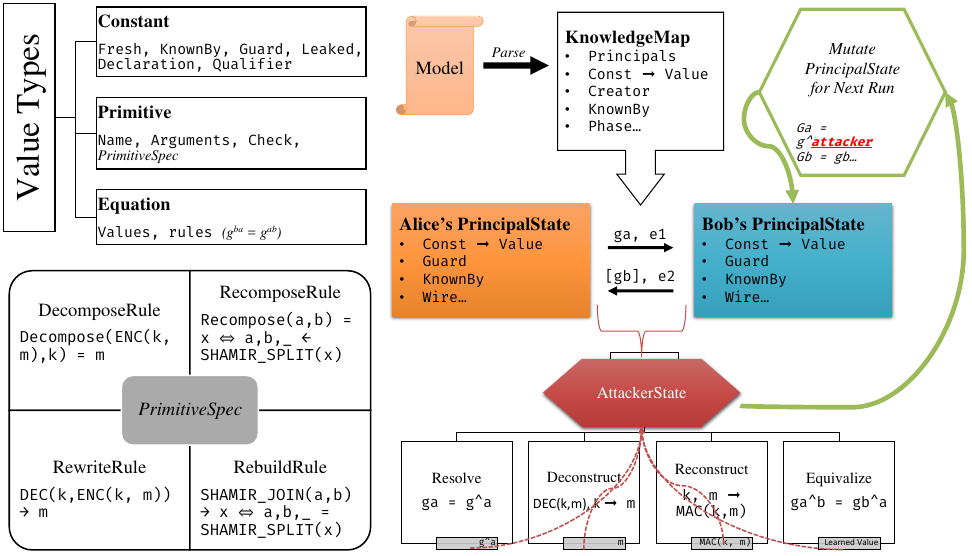
\includegraphics[scale=.30]{verifpal-internals}
    \caption{All credits to Nadim Kobeissi.}
  \end{figure}
  \begin{multicols}{2}
  \begin{enumerate}
    \item{Gather values;}
    \item{Populate attacker state;}
    \item{Apply transformations;}
    \item{Prepare next mutations;}
    \item{Mutate protocol executions.}
  \end{enumerate}
  \end{multicols}
\end{frame}

\section{Case studies}
\framecard{Case studies:\\Diffie-Hellman and\\Needham-Schroeder Public Key}

\begin{frame}{Case studies}
  Two case studies:
  \begin{itemize}
    \item{Diffie-Hellman}
    \item{Needham-Schroeder Public Key}
  \end{itemize}
  
  \vskip 1cm
  
  \begin{block}{Source code}
  The source code of the case studies in the next few slides is available on github \cite{CaseStudies}.
  \end{block}
\end{frame}

\subsection{Diffie-Hellman}
\begin{frame}[fragile]{Diffie-Hellman}
  \begin{columns}[c]
    \column{0.6\textwidth}
    We will consider three versions:
    \begin{itemize}
      \item{Anonymous}
      \item{Ephemeral}
      \item{Perfect Forward Secrecy Ephemeral}
    \end{itemize}
    \column{0.4\textwidth}
    \begin{figure}[t]
      \setmscoptions
      \begin{msc}{}
      \setmscscale{.5} 
      
      \declinst{client}{}{Client}
      \declinst{server}{}{Server}
      
      \action*{\parbox{3.5cm}{\centering
          Knows $g, p$\\
          $c \in \Z$\\
          $g_c := \modexp{g}{c}{p}$
      }}{client}

      \nextlevel[5]
      \mess{$g_c$}{client}{server}
      \nextlevel

      \action*{\parbox{3.5cm}{\centering
          Knows $g, p$\\
          $s \in \Z$\\
          $g_s := \modexp{g}{s}{p}$\\
          $\skey{c} := \modexp{g_c}{s}{p}$
      }}{server}

      \nextlevel[6]
      \mess{$g_s$}{server}{client}
      \nextlevel

      \action*{\parbox{3.5cm}{\centering
          $\key{cs} := \modexp{g_s}{c}{p}$
      }}{client}
      \nextlevel

      \end{msc}
      \centering
    \end{figure}
\end{columns}
\end{frame}

\begin{frame}[fragile]{Anonymous Diffie-Hellman}
  Straightforward implementation.

  \vskip 0.25cm

  To store keys (for message exchanges):
  \begin{itemize}
    \lstset{language=tamarin}
    \item{Tamarin $\to$ Persistent fact: \lstinline{!ClientKey(k)}}
    \lstset{language=proverif}
    \item{Proverif $\to$ Table: \lstinline{insert ClientKeyTable(k);}}
  \end{itemize}

  \lstset{basicstyle=\scriptsize\ttfamily}
  \begin{columns}[onlytextwidth,t]
    \hspace*{-.60cm}
    \begin{column}{0.5\paperwidth}
    \centering
    \lstset{language=tamarin}
      \begin{lstlisting}
/* Send a message from client to server */
rule ClientSendMessage:
    [
      Fr(~m),
      !ClientKey(k)
    ]
  --[ ClientSentMessage(k, ~m) ]->
    [ Out(senc(<'CtoS', ~m>, k)) ]
      \end{lstlisting}
    \end{column}

    \begin{column}{0.5\paperwidth}
      \centering
      \lstset{language=proverif}
      \begin{lstlisting}
let ClientSendsMessage() =
  (* Generate fresh message m *)
  new m: Plaintext;

  (* Get client key from table *)
  get ClientKey(k) in
  event ClientSentMessage(m, k);
  out(io, enc(m, k));
  0.
      \end{lstlisting}
    \end{column}
  \end{columns}
\end{frame}

\begin{frame}[fragile]{Epehemeral Diffie-Hellman}
  Server half key needs to be authenticated:
  \begin{itemize}
    \item{Tamarin $\to$ private channel with passive attacker:
      \begin{lstlisting}[language=tamarin]
rule CertificateExchange:
    [ CertificateOut(x) ] --> [ CertificateIn(x), Out(x) ]
      \end{lstlisting}
    }
    \item{Proverif $\to$ table (output every value we insert):
    \begin{lstlisting}[language=proverif]
table AuthenticatedValueTable(G).

let Server() =
  ...
  insert AuthenticatedValueTable(g_r);
  out(io, g_r);
...
    \end{lstlisting}
    }
    \item{Verifpal $\to$ guarded variables (between square brackets):
    \begin{lstlisting}[language=verifpal]
Server -> Client: [g_s], c1
    \end{lstlisting}
    }
  \end{itemize}
\end{frame}

\begin{frame}[t,fragile,allowframebreaks]{PFS Ephemeral Diffie-Hellman}
  We model the leakage of ephemeral keys:
  \begin{itemize}
    \item{Tamarin $\to$ Fact for the ephemeral key, rule to output it:
      \begin{lstlisting}[language=tamarin]
rule RevealClientEphemeralKey:
    [ ClientEphemeralKey(c) ]
  --[ RevealedClientEphemeralKey(c) ]->
    [ Out(c) ]
      \end{lstlisting}
      Use lemma timepoints to leak the value after a certain event;
    }
    \lstset{language=proverif}
    \item{Proverif $\to$ create a process in \lstinline{phase 1}:
    \begin{lstlisting}
let PostRevealClientEphemeralKey =
  phase 1;
  (* Get the client's ephemeral key and output it *)
  get ClientEphemeralKeyTable(c) in
  out(io, c);
  event PostRevealedClientEphemeralKeyTable(c);
  0.
    \end{lstlisting}
    }
    \lstset{language=verifpal}
    \item{Verifpal $\to$ very similar to Proverif, using \lstinline{phase} and \lstinline{leaks}:
    \begin{lstlisting}
phase [1]

principal Client [
  leaks c
]

principal Server [
  leaks s
]
\end{lstlisting}
    }
  \end{itemize}
\end{frame}

\subsection{Needham-Schroeder Public Key}
\begin{frame}{Needham-Schroeder Public Key}
  \begin{columns}[onlytextwidth,c]
    \column{0.6\textwidth}
    We will consider two versions of the (simplified) Needham-Schroeder Public Key protocol:
    \begin{itemize}
      \item{Flawed}
      \item{Fixed}
    \end{itemize}
    \column{0.4\textwidth}
    \begin{figure}[t]
      \setmscoptions
      \setlength{\instdist}{2cm}
      \begin{msc}{}
      \setmscscale{.5} 
      
      \declinst{alice}{}{Alice}
      \declinst{bob}{}{Bob}
      
      \action*{\parbox{3.5cm}{\centering
          Knows $\skey{A}, \pkey{A}$\\
          Knows $\pkey{B}$
      }}{alice}

      \action*{\parbox{3.5cm}{\centering
          Knows $\skey{B}, \pkey{B}$\\
          Knows $\pkey{A}$
      }}{bob}
      \nextlevel[4]

      \action*{\parbox{3.5cm}{\centering
          Generates $N_A$
      }}{alice}

      \nextlevel[3]    
      \mess{$\enc{N_A, A}{\pkey{B}}$}{alice}{bob}
      \nextlevel


      \action*{\parbox{3.5cm}{\centering
          Generates $N_B$
      }}{bob}

      \nextlevel[3]
      \mess{$\enc{N_A, N_B}{\pkey{A}}$}{bob}{alice}
      \nextlevel[2]
      \mess{$\enc{N_B}{\pkey{B}}$}{alice}{bob}

      \end{msc}
      \centering
    \end{figure}
  \end{columns}
\end{frame}

\begin{frame}[t,allowframebreaks]{Bibliography}
  \printbibliography
\end{frame}


%% -------------------------------------------------------------------------------- %%
%% Preset slides start here                                                         %%
%% -------------------------------------------------------------------------------- %%

\section{Colors}

\begin{frame}{Colors}

For this template we defined four colors, following the Style Manual of the University of Udine:
\begin{itemize}
\item \textcolor{white}{\marker{\texttt{UniOrange}}}
\item \textcolor{white}{\marker[UniBlue]{\texttt{UniBlue}}}
\item \textcolor{white}{\marker[UniBrown]{\texttt{UniBrown}}}
\item \textcolor{white}{\marker[UniGold]{\texttt{UniGold}}}
\end{itemize}

\vskip 0.5cm

You can use these colors as you want in your presentation. For example, you can \textbf{\textcolor{UniGold}{color the text in gold}} by writing \texttt{\textbackslash\{UniGold\}\{my gold text\}}.

\vskip 0.5cm

We also redefined many of the most common \LaTeX{} and Beamer commands, like \texttt{itemize}, \texttt{block}, etc. You will see samples of these commands in the following slides.

\end{frame}

\section{Blocks}

\begin{frame} 
\frametitle{This is a page with a title and a subtitle} 
\framesubtitle{And also some blocks.} 
\begin{block}{Goal of the mission}
Shoot in the Death Star's exhaust port and destroy it before the it can fire on the Rebel base.
\end{block} 
\begin{alertblock}{Take care!}
TIE Fighters may chase you while approaching the target.
\end{alertblock} 
\begin{exampleblock}{Use the force you must}
Remember your training with Obi-Wan, and use the Force to make the perfect shoot.
\end{exampleblock} 

\end{frame}

\section{Enumerates, itemizes and description}

\subsection{Enumerates and itemizes}

\begin{frame}{Enumerates and itemizes}

This is an example of \texttt{itemize}.
\begin{itemize}
	\item A long time ago in a galaxy far, far away...
\end{itemize}
And this is an example of \texttt{enumerate}.

\begin{enumerate} 
  \item Go to the Death Star.
  \item Find the exhaust port.
  \item Make the perfect shot.
  \item Become an hero.
\end{enumerate}
\end{frame}

\subsection{Description}

\begin{frame}[fragile]
\frametitle{Description}
This is an example of \texttt{description}.

\begin{description}
\item<2->[Vader] \emph{I am} your father.
\item<1->[Luke] No. No! That's not true! \textbf{That's impossible!}
\end{description}

\begin{uncoverenv}<3>
  \vskip 0.5cm
  And while we're here, let's have a look to \texttt{verbatim} as well, to see how we made items appear in arbitrary order:
  \vskip 0.5cm
  \begin{verbatim}
\begin{description}
  \item<2->[This is the first item] one
  \item<1->[This is the second item] two
\end{description}
  \end{verbatim}
\end{uncoverenv}

\end{frame}

\section{Maths}

\begin{frame}{Maths}
A formula will look like this: 
\begin{center}
 $x^2 + y^2 = z^2$
\end{center}

You can number equations as well:
\begin{equation}
1+1=2
\end{equation}

\begin{equation}
1+1=2 \tag{custom label!}
\end{equation}

\vskip 0.5cm

If you want to use the default \LaTeX{} math fonts, just go to \texttt{beamerfontthemeuniud.sty} and uncomment the line containing `\texttt{\textbackslash usefonttheme[onlymath]\{serif\}}'.

\end{frame}

\begin{frame}{Theorems}

The usual \texttt{theorem}, \texttt{corollary}, \texttt{definition}, \texttt{definitions}, \texttt{fact}, \texttt{example} and \texttt{examples} blocks are available as well.

\begin{theorem}
There exists an infinite set.
\end{theorem}
\begin{proof}
This follows from the axiom of infinity.
\end{proof}
\begin{example}[Natural Numbers]
The set of natural numbers is infinite.
\end{example}

\end{frame}

\section{Other blocks}

\begin{frame}{Other blocks}

Here we display examples of \texttt{abstract}, \texttt{verse}, \texttt{quotation}, and \texttt{quote}.

\vskip 0.5cm

\begin{abstract}
This is an abstract.
\end{abstract}
\begin{verse}
This is a verse.
\end{verse}
\begin{quotation}
This is a quotation.

\raggedleft -Han Solo
\end{quotation}
\begin{quote}
A quote this is.

\raggedleft -Yoda
\end{quote}

\end{frame}

\section{Bibliography and Publications}
\begin{frame}[fragile]
\frametitle{Bibliography}

You can cite an article
\begin{itemize}
  \item{}
\end{itemize}

\vskip 0.5cm
Look at the code of the following slide to see how to automatically split the bibliography on many slides. You can also use \texttt{\textbackslash nocite\{*\}} to display the non-cited publications as well.

\end{frame}

\begin{frame}[t,allowframebreaks]
\frametitle{Bibliography}

\nocite{*} % will display the non-cited publications as well. Useful for a publication list.

\printbibliography

\end{frame}

\section{Bonus Commands}

\begin{frame}[fragile]
\frametitle{Framecard}

You can display a frame with a colored background and a huge text in the center using the command \texttt{\textbackslash framecard}.
\vskip 0.5cm 
For example, you can write:
\begin{verbatim}
\framecard{A SECTION\\TITLE}
\end{verbatim}

This will display a frame with a orange background and the phrase "A SECTION TITTLE" in the center. You can also use a custom color with \texttt{\textbackslash framecard}:
\begin{verbatim}
\framecard{A SECTION\\TITLE}
\framecard[UniBlue]{A SECTION TITLE\\
WITH A CUSTOM COLOR}
\end{verbatim}
You can see the results of the commands above in the following slides.

\end{frame}

\framecard{A SECTION\\TITLE}
\framecard[UniBlue]{A SECTION TITLE\\WITH A CUSTOM COLOR}

\begin{frame}[fragile]
\frametitle{Framepic}

You can display a frame with a background image using the command \texttt{\textbackslash framepic}. The image will be \textbf{adapted vertically} to fit the the frame. 

For example, you can write:
\begin{verbatim}
\framepic{graphics/darth}{
	\framefill
    \textcolor{white}{Luke,\\I am your supervisor}
    \vskip 0.5cm
}
\end{verbatim}

Alternatively, to make the background 50\% transparent, you can write \texttt{\textbackslash framepic[0.5]\{graphics/darth\}...}


You can see the results of the commands above in the following slides.

\end{frame}


\framepic{graphics/darth}{
	\framefill
    \textcolor{white}{Luke,\\I am your supervisor}
    \vskip 0.5cm
}

\framepic[0.5]{graphics/darth}{
	\vfill
    \begin{flushright}
    \textcolor{red}{\textbf{Right-aligned text with\\Semi-transparent background}}
    \end{flushright}	
}

\begin{frame}[t,fragile,allowframebreaks]
\frametitle{Other bonus commands}

We provide two other bonus commands:
\begin{description}
\item[\texttt{pdfnewline}] you can use \texttt{\textbackslash pdfnewline} to avoid the annoying \texttt{hyperref} related warnings when using newlines in the document's title, author, etc. For example, in this presentation the author is defined as:
\begin{verbatim}
\author[Luke Skywalker]{
  Luke Skywalker, Ph.D.
  \pdfnewline
  \texttt{luke.skywalker@uniud.it}
}
\end{verbatim}
\item[\texttt{marker}] you can use \texttt{\textbackslash marker} to highlight some text. The default color is \marker{orange}, but you can also \marker[UniBlue]{use a custom color}. For example:
\begin{verbatim}
\marker{Default color}
\marker[UniBlue]{Custom Color}
\end{verbatim}
\item[\texttt{framefill}] you can use \texttt{\textbackslash framefill} to put the text at the bottom of a slide by filling all the vertical space.
\end{description}

\end{frame}

\end{document}